\mychapter{2}{BAB II \\ GAMBARAN UMUM PERUSAHAAN}

\section{Sejarah Perusahaan}

Mulai beroperasi pada tahun 2006 dengan melayani katering harian untuk pelanggan disekitar Karawang, 
tanpa harus ada suatu badan hukum. Karena ada permintaan yang lebih besar dari pabrik dengan jumlah porsi 
yang besar, maka pada tahun 2016 dibentuk suatu badan hukum PT. Boga Pangan Sentosa (PT. BPS). 
Sesuai dengan visi dan misi dari PT. BPS, perusahaan akan menjadi suatu perusahaan catering yang 
terkemuka di Indonesia dengan mengutamakan kualitas dengan cita rasa yang lezat dan higenis. 

PT. BPS memiliki layanan yang dapat disesuaikan untuk berbagai jenis acara perusahaan atau 
pribadi. Mulai dari menyediakan sarapan, makan siang, dan makan malam, 
PT. BPS menawarkan seluruh penawaran termasuk layanan yang ramah dan profesional. 
Dalam hal memberi makan karyawan, dibutuhkan katering yang dapat percaya untuk melakukan 
pekerjaan dengan benar.  PT. BPS menawarkan pilihan makanan yang disesuaikan yang dikirim 
atau disajikan tepat waktu. Kebutuhan setiap bisnis dari pelanggan adalah unik dan memastikan 
semuanya terpenuhi. Kualitas adalah bahan pokok dalam setiap menu yang dibuat dan anggaran bisnis 
dari pelanggan akan disesuaikan. Hal ini berarti tenaga kerja yang lebih bahagia, sehat dan produktif 
demi meningkatkan produktifitas bisnis pelanggan akan menjadi perhatian 
PT. BPS dalam menyajikan hidangan menu setiap harinya dan memberikan pelayanan yang terbaik.\

\section{Visi Perusahaan}

Visi dari PT. BPS adalah menjadi perusahaan katering industri kelas dunia terbesar 
di Indonesia dengan memberikan 
pelayanan yang berkualitas dan berkelas dalam setiap hidangan yang disajikan.

\section{Misi perusahaan}
\begin{itemize}
\item Memberikan pelayanan terbaik kepada pelanggan secara konstan 
dan terus meningkatkan kualitas dari kritik dan saran yang diberikan pelanggan,
\item Memberikan kualitas dan cita rasa yang berkelas dan konsiten. 
\item Komitmen pada hal kualitas, kebersihan dan waktu, terus 
berinovasi untuk memberikan pengalaman lebih pada pelanggan dalam dunia katering, 
\item Menjadi partner yang dapat memberikan solusi jika perusahaan membutuhkan pelayanan katering.
\end{itemize}

\section{Nilai Prinsip Perusahaan}
 Perusahaan memiliki tiga nilai yang menjadi prinsip dalam pengembangan bisnis yaitu higienis, 
 berkualitas, dan pelayanan. Dapur perusahaan dikelola secara higienis dan professional guna memastikan 
 keamanan pekerja dan kesehatan makanan. Selain itu, kualitas bahan makanan yang terjamin dan harga terjangkau. 
 PT. BPS tetap menjaga kualitas agar cita rasa mekanan tetap konsisten. Memberikan pelayanan yang terbaikSemua 
 kritik dan masukan dari pelanggan akan menjadi masukan bagi perusahaan

 \section{Logo Perusahaan}
 PT. BPS memiliki logo yang sederhana dan mudah diingat oleh pelanggan. 
 Logo mencerminkan arti yang sangat penting dan menjadi \emph{brand} yang harus terus dikembangkan. 
 Pada logo BPS terdapat warna merah yang melambangkan berani untuk 
 melangkah maju dan terus berinovasi untuk mencapai visi yang dirancang. 
 Tulisan BPS pada logo melambangkan singkatan dari Boga Pangan Sentosa.

\begin{figure}[htbp]
\begin{center}

\includegraphics{img/logo-bps.png}
\caption{Logo PT. Boga Pangan Sentosa.}
\label{gambar:logo-bps}
\end{center}
\end{figure}

\pagebreak

\section{Struktur Organisasi Perusahaan}

Suatu organisasi membutuhkan suatu struktur agar semua dapat berlangsung dengan lancar dan jelas. 
Tugas yang dikerjakan setiap divisi dan pertanggung-jawaban setiap divisi kepada atasan.

\subsection{Struktur Organisasi }

\begin{figure}[htbp]
    \begin{center}
    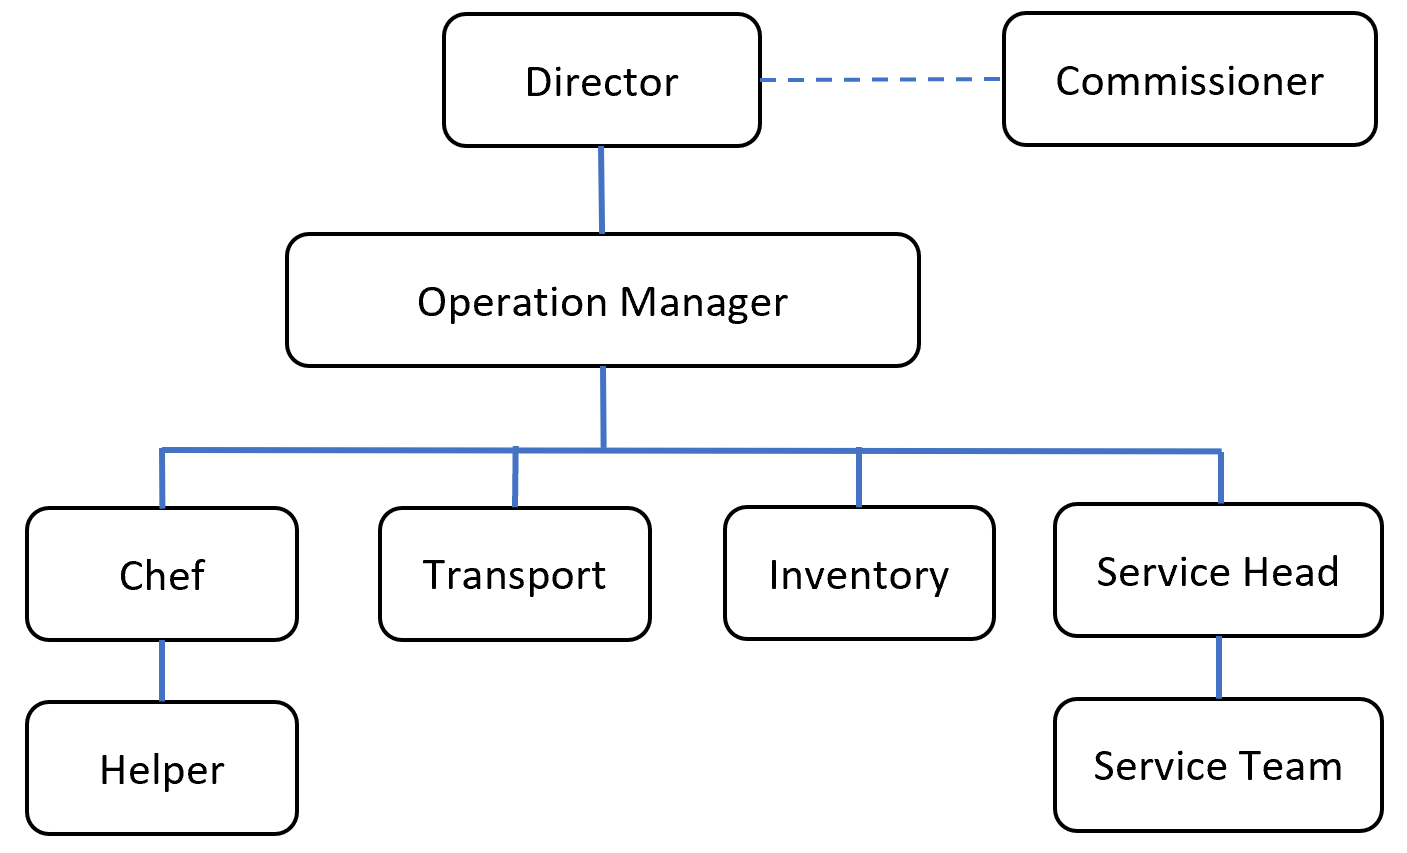
\includegraphics[width=10cm]{img/struktur-org.png}
    \caption{Struktur Perusahaan.}
    \label{gambar:struktur-org}
    \end{center}
\end{figure}

\subsection{Tugas dan Tanggung Jawab}
Struktur organisasi yang dimiliki oleh PT. BPS terbagi atas beberapa bagian yang memiliki 
fungsinya masing-masing. 
Berikut adalah penjelasan singkat tugas dan tanggung jawab dari masing-masing posisi divisi sebagai berikut:

\begin{enumerate}
    \item  \emph{Director}
        \begin{itemize}
        \item mengawasi dan mengarahkan jalannya perusahaan sesuai dengan visi dan misi.
        \item Memantau kerja dari operational manager.
        \end{itemize}
    \item \emph{Commissioner} 
        \begin{itemize}
        \item Mengawasi jalannya perusahaan.
        \item Memberikan arahan kepada director jika diperlukan.
        \end{itemize}
    \item \emph{Operational Manager}
        \begin{itemize}
        \item Bertanggung jawab untuk memenuhi kebutuhan dari pelanggan.
        \item Mengelola pemasukan dan pengeluaran perusahaan.
        \end{itemize}
    \item \emph{Chef dan Helper}
        \begin{itemize} 
        \item Bertanggung jawab memproduksi menu hidangan sesuai dengan standar yang ditetapkan perusahaan.
        \item Bertanggung jawab terhadap kepatuhan penggunaan standar resep.
        \item Bertanggung jawab terhadap hasil olahan menu.
        \item Membantu koki untuk mempersiapkan bahan dan peralatan.
        \end{itemize}
    \item \emph{Transport}
        \begin{itemize} 
        \item Mengantar makanan sampai ke tujuan.
        \item Memastikan kendaraan siap untuk beroperasi.
        \item Membuat laporan dan evaluasi terhadap aktivitas perjalanan.
        \item \emph{Inventory} 
        \item Memonitor dan mengelola proses pemenuhan order secara berkala.
        \item Bertanggung jawab dengan jumlah persediaan barang.
        \item Mengontrol masuk dan keluarnya barang dari gudang persediaan.
        \end{itemize}
    \item \emph{Service}
    \begin{itemize}
    \item Melayani pelanggan dengan ramah.
    \item Memberikan pelayanan dengan cepat.
    \end{itemize}
\end{enumerate}

\section{Produk Perusahaan}

\subsection{Katering Umum}

PT. BPS berpengalaman pada layanan katering umum seperti pada perayaan khitanan, 
arisan, ulang tahun, dan perayaan lainnya. PT. BPS siap menyajikan hidangan terbaik dan layanan yang memuaskan. 
Beragam pelanggan dengan berbagai perayaan kegiatan telah mempercayakan PT. BPS.

\subsection{katering Kantor}
Beberapa perusahaan mengutamakan efisiensi waktu pada saat jam istirahat. 
Waktu yang terbuang dan rasa lelah ketika harus pergi keluar kantor untuk makan 
siang bisa ditangani dengan berlangganan paket makan siang. Dengan latar belakang tersebut, 
PT. BPS menawarkan sebuah solusi kepada perusahaan dalam hal jasa katering dengan berbagai 
macam gaya makanan sesuai dengan selera pelanggan. 
PT. BPS siap melayani perusahaan dan menjadi mitra penyedia katering.

\subsection{Katering Industri/Pabrik}
Fenomena pada saat makan siang di kawasan industri, karyawan harus antri dan berdesakan sehingga 
tidak dapat menikmati menu makan siang. Hal ini tidak perlu terjadi apabila kebutuhan makan siang 
karyawan pabrik dipercayakan kepada pihak yang berpengalaman. PT. BPS siap memberikan solusi menu makan 
siang sesuai dengan kebutuhan pabrik dan perusahaan dengan karyawan dalam jumlah besar. 
Cara pengemasan pelayanan pada industri berbeda dari acara pribadi.  
Layanan catering yang diberikan kepada bisnis pelanggan dengan standar tinggi dan profesional. 
PT. BPS memelihara catatan layanan yang sangat baik, 
tim profesional dan terlatih untuk melayani semua jenis katering Industri.

\section{Daftar Pelanggan Industri}

Sejak tahun PT. BPS berbadan hukum, sebagian dari pelanggan industri besar adalah:
\begin{multicols}{2}
\begin{itemize}
\item PT. HM Sampoerna Tbk.
\item PT. Philip Morris Indonesia
\item PT. JTEKT Indonesia
\item PT. Piolax Indonesia
\item PT. Nici Indonesia
\item PT. Yangtze Optical Fibre Indonesia (PT. YOFI)
\item PT. Essence Indonesia (PT. IFF)
\item PT. Tsuruta Indonesia
\item PT. Furukawa Automotive Systems Indonesia (PT. FASI)
\item PT. Surya Rengo Containers (PT. SRC)
\item PT. Hiruta Kogyo Indonesia
\item PT. Marugo Rubber Indonesia
\end{itemize}
\end{multicols}